\newcommand{\lecturetitle}[1]{
  \title{01204211 Discrete Mathematics \\ #1}
  \author{Jittat Fakcharoenphol}
  \frame{\titlepage}
}
\newcommand{\Mod}{\,\bmod\,}

\lecturetitle{Lecture 8a: Linear systems of equations} 

\begin{frame}
  \frametitle{Linear algebra}

  Linear algebra studies 
  \begin{itemize}
  \item matrices and operations with matrices
  \item systems of linear equations
  \item linear transformations
  \item linear spaces (and their structures)
  \end{itemize}
\end{frame}

\begin{frame}
  \frametitle{Why?}

  \begin{itemize}
  \item Lots of applications.
  \item Interesting perspectives.
  \end{itemize}
\end{frame}

\begin{frame}\frametitle{A linear system of equations}
  Let's start with a simple example with 2 variables:

  \[
  \begin{array}{rcl}
  5x + 10y &=& 5 \\
  x - 3y &=& 11
  \end{array}
  \]

  How would you solve it?

  \pause

  Using basic techniques you learned from high school, you may
  multiply the second equation with $5$ and subtract it to the first
  equation; yielding:

  \[
    5x + 10y - (5x - 5\cdot 3y) =
    \pause 25y = 5 - 5\cdot 11 =
    \pause -50
  \]

  \pause

  Then you can conclude that $y=-2$.  Substitute it to one of the
  equation, you can find out the value of $x$.

\end{frame}

\begin{frame}
  \frametitle{Gaussian elimination (1)}
  Let's consider a system with 3 variables:

  \[
  \begin{array}{rcrcrcl}
    2x_1 & + & 4x_2 & + & 3x_3 & = & 7 \\
    x_1 & + &  &  & 5x_3 & = & 12 \\
    4x_1 & + & 2x_2 & + & 3x_3 & = & 10
  \end{array}
  \]

  \vspace{2in}

\end{frame}

\begin{frame}
  \frametitle{Gaussian elimination (2)}
  Let's consider another system with 3 variables:

  \[
  \begin{array}{rcrcrcl}
    2x_1 & + & 4x_2 & + & 3x_3 & = & 7 \\
    x_1 & + &  &  & 5x_3 & = & 12 \\
    3x_1 & + & 8x_2 & + & x_3 & = & 10
  \end{array}
  \]

  \vspace{2in}

\end{frame}

\begin{frame}
  \frametitle{A closer look: 1st perspective}

  Consider
  \[
  \begin{array}{rcl}
  5x + 10y &=& 5 \\
  x - 3y &=& 11
  \end{array}
  \]
  Each equation (row) constraints certain values of $x$ and $y$.
  \vspace{2.5in}
\end{frame}

\begin{frame}
  \frametitle{``Combining'' two rows}
  Let's focus only on coefficients.
  This is how we obtain the third equation:
  \[
  \begin{array}{rccll}
    ( & 5, & 10 & ) & =\uv_1\\
    ( & 1, & -3 & ) & =\uv_2\\
    \pause
    ( & 0, & 25 & ) & =\uv_1 - 5\cdot \uv_2
  \end{array}
  \]
  \pause
  The third equation is a ``combination'' of the other two rows.  In fact, it is a \textcolor{red}{\bf linear combination} of the first two.
  \pause
  
  Can you obtain $(0,1)$ from $\uv_1$ and $\uv_2$?
  \pause
  
  Yes,
  \[
  0.2\cdot \uv_1 -\uv_2 = (0,1).
  \]
  
  It turns out that you can obtain any $(a,b)$ from $\uv_1$ and $\uv_2$.
\end{frame}

\begin{frame}
  \frametitle{A closer look: 1st perspective (more example)}

  Consider
  \[
  \begin{array}{rcrcrcl}
    2x_1 & + & 4x_2 & + & 3x_3 & = & 7 \\
    x_1 & + &  &  & 5x_3 & = & 12 \\
    4x_1 & + & 2x_2 & + & 3x_3 & = & 10
  \end{array}
  \]
  What are the row vectors?

  \vspace{2in}
\end{frame}

\begin{frame}
  \frametitle{A closer look: 2nd perspective}
  We rewrite the system as

  \[
  \begin{bmatrix}
    5 \\ 1
  \end{bmatrix}
  \cdot x +
  \begin{bmatrix}
    10 \\ -3
  \end{bmatrix}
  \cdot y
  =
  \begin{bmatrix}
    5 \\ 11
  \end{bmatrix}
  \]

  \pause

  Now, the goal is to find $x$ and $y$ satisfying this ``vector'' equation.

  \pause

  But if we change our focus to the vectors, we can see that we have 3 vectors:

  \[
  \vv_1=
  \begin{bmatrix}
    5 \\ 1
  \end{bmatrix},
  \ \ \
  \vv_2 = 
  \begin{bmatrix}
    10 \\ -3
  \end{bmatrix},
  \ \ \
  {\bm b} =
  \begin{bmatrix}
    5 \\ 11
  \end{bmatrix}
  \]

  \pause

  and with $x$ and $y$, we now see that ${\bm b}$ is a \textcolor{red}{\bf linear combination} of $\vv_1$ and $\vv_2$.
  
  Finding $x$ and $y$ is essentially checking if ${\bm b}$ is a linear combination of $\vv_1$ and $\vv_2$.
\end{frame}


\begin{frame}
\frametitle{Example 2: a linear system with 2 variables}
  {\small
  \[
  \begin{array}{rcrcrcl}
    x & + & y & = & 7 \\
    x & - & 2y & = & 13 \\
  \end{array}
  \]
  }

  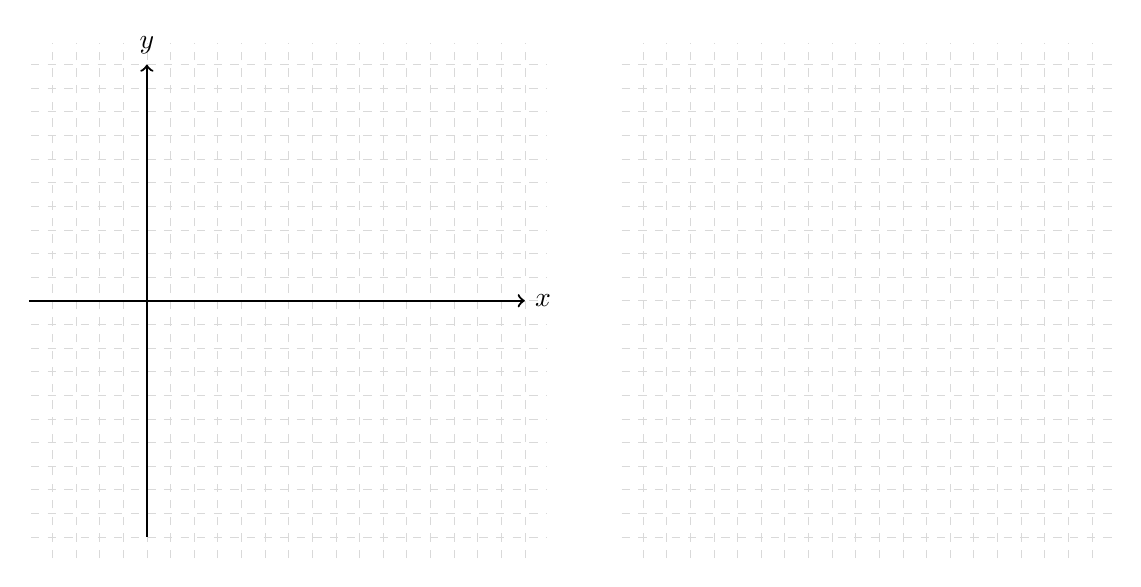
\begin{tikzpicture}[scale=0.3]
    \draw[help lines, color=gray!30, dashed] (-10.9,-10.9) grid (10.9,10.9);
    \draw[->,thick] (-11,0)--(10,0) node[right]{$x$};
    \draw[->,thick] (-6,-10)--(-6,10) node[above]{$y$};

    \draw[help lines, color=gray!30, dashed] (14.1,-10.9) grid (34.9,10.9);
  \end{tikzpicture}

\end{frame}


\begin{frame}
\frametitle{Example 3: a linear system with 2 variables}
  {\small
  \[
  \begin{array}{rcrcrcl}
    2x & + & y & = & 5 \\
    4x & + & 2y & = & 10 \\
  \end{array}
  \]
  }

  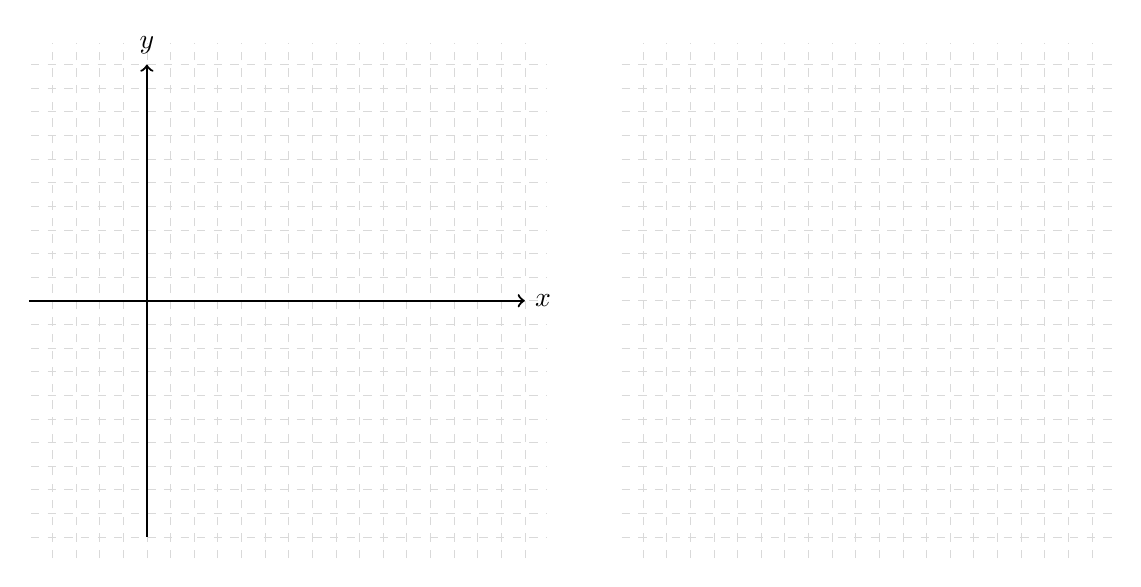
\begin{tikzpicture}[scale=0.3]
    \draw[help lines, color=gray!30, dashed] (-10.9,-10.9) grid (10.9,10.9);
    \draw[->,thick] (-11,0)--(10,0) node[right]{$x$};
    \draw[->,thick] (-6,-10)--(-6,10) node[above]{$y$};

    \draw[help lines, color=gray!30, dashed] (14.1,-10.9) grid (34.9,10.9);
  \end{tikzpicture}

\end{frame}

\begin{frame}
\frametitle{Example 4: a linear system with 2 variables}
  {\small
  \[
  \begin{array}{rcrcrcl}
    x & + & 3y & = & 6 \\
    0.5\cdot x & + & 1.5\cdot y & = & 9 \\
  \end{array}
  \]
  }

  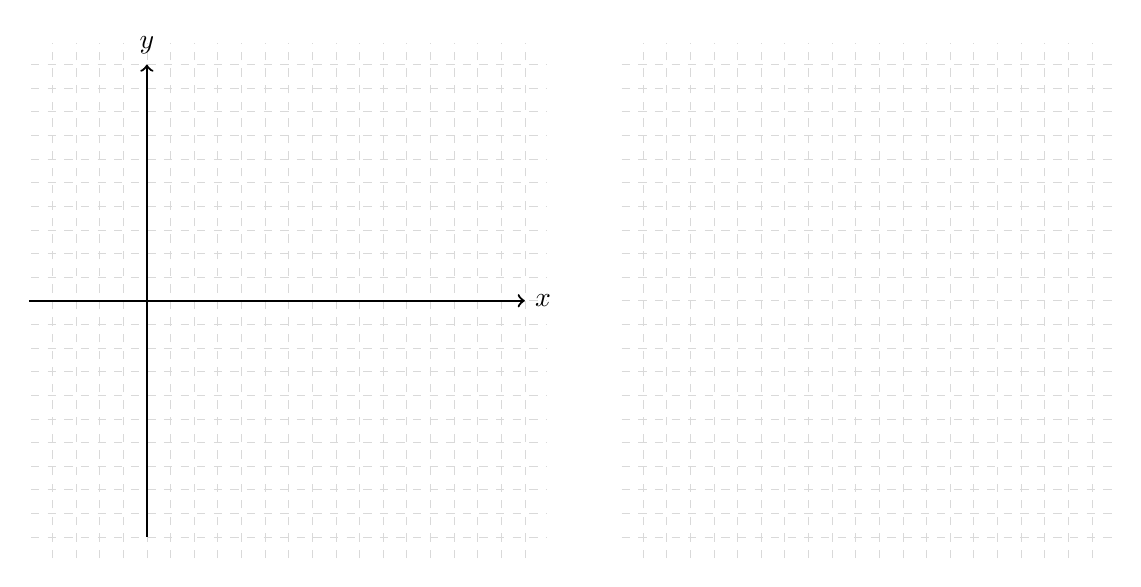
\begin{tikzpicture}[scale=0.3]
    \draw[help lines, color=gray!30, dashed] (-10.9,-10.9) grid (10.9,10.9);
    \draw[->,thick] (-11,0)--(10,0) node[right]{$x$};
    \draw[->,thick] (-6,-10)--(-6,10) node[above]{$y$};

    \draw[help lines, color=gray!30, dashed] (14.1,-10.9) grid (34.9,10.9);
  \end{tikzpicture}

\end{frame}

\begin{frame}
  \frametitle{A linear system with 3 variables}
  Let's consider a system with 3 variables:

  \[
  \begin{array}{rcrcrcl}
    2x_1 & + & 4x_2 & + & 3x_3 & = & 7 \\
    x_1 & + &  &  & 5x_3 & = & 12 \\
    4x_1 & + & 2x_2 & + & 3x_3 & = & 10
  \end{array}
  \]

  \vspace{2in}

\end{frame}

\begin{frame}
  \frametitle{Row perspective}

  {\tiny
  \[
  \begin{array}{rcrcrcl}
    2x_1 & + & 4x_2 & + & 3x_3 & = & 7 \\
    x_1 & + &  &  & 5x_3 & = & 12 \\
    4x_1 & + & 2x_2 & + & 3x_3 & = & 10
  \end{array}
  \]
  }

  Each equation becomes a {\bf plane} in 3 dimensional space.

  \vspace{2.5in}
  
\end{frame}

\begin{frame}
  \frametitle{Row perspective: the goal of Gaussian Elimination}

  From vectors:
  \[
  (2,4,3), \ \ \ (1,0,5), \ \ \ (4,2,3)
  \]

  We want to linearly combine them to obtain
  \[
  (1,0,0), \ \ \ (0,1,0), \ \ \ (0,0,1)
  \]

  \pause

  In other words,
  what are the possible linear combinations of 
  \[
  (2,4,3), \ \ \ (1,0,5), \ \ \ (4,2,3)
  \]

\end{frame}


\begin{frame}
  \frametitle{Column perspective}
  From
  {\tiny
  \[
  \begin{array}{rcrcrcl}
    2x_1 & + & 4x_2 & + & 3x_3 & = & 7 \\
    x_1 & + &  &  & 5x_3 & = & 12 \\
    4x_1 & + & 2x_2 & + & 3x_3 & = & 10
  \end{array},
  \]
  }
  we rewrite the system as

  \[
  \begin{bmatrix}
    2 \\ 1 \\ 4
  \end{bmatrix}
  \cdot x_1 +
  \begin{bmatrix}
    4 \\ 0 \\ 2
  \end{bmatrix}
  \cdot x_2 +
  \begin{bmatrix}
    3 \\ 5 \\ 3
  \end{bmatrix}
  \cdot x_3 +
  =
  \begin{bmatrix}
    7 \\ 12 \\ 10
  \end{bmatrix}.
  \]

  Our goal is to find a way to linear combine 3 vectors to obtain
  \[
  \begin{bmatrix}
    7 \\ 12 \\ 10
  \end{bmatrix}.
  \]

  \pause

  In other words, the vector ${\bm b}$, for a successful Gaussian
  Elimination, should be in the set of all possible linear combinations
  of the 3 column vectors.
\end{frame}

\begin{frame}
  \frametitle{More example}
  Let's consider another system with 3 variables:

  \[
  \begin{array}{rcrcrcl}
    2x_1 & + & 4x_2 & + & 3x_3 & = & 7 \\
    x_1 & + &  &  & 5x_3 & = & 12 \\
    3x_1 & + & 8x_2 & + & x_3 & = & 10
  \end{array}
  \]

  \vspace{2in}

\end{frame}

\begin{frame}
  \frametitle{More example 2}
  Let's consider another system with 3 variables:

  \[
  \begin{array}{rcrcrcl}
    2x_1 & + & 4x_2 & + & 3x_3 & = & 7 \\
    x_1 & + &  &  & 5x_3 & = & 12 \\
    4x_1 & + & 2x_2 & + & 3x_3 & = & 10 \\
    5x_1 & + & 2x_2 & + & 8x_3 & = & 22
  \end{array}
  \]

  \vspace{2in}

\end{frame}

\begin{frame}
  \frametitle{More failed example 3}
  Let's consider the last system with 3 variables:

  \[
  \begin{array}{rcrcrcl}
    2x_1 & + & 4x_2 & + & 3x_3 & = & 7 \\
    x_1 & + &  &  & 5x_3 & = & 12 \\
    2x_1 & + &  &  & 10x_3 & = & 24 \\
  \end{array}
  \]

  \vspace{2in}

\end{frame}

\begin{frame}
  \frametitle{More failed example 3 (cont.)}
  The last equation (constraint) can be derived from the other two.
  
  \[
  \begin{array}{rcrcrcl}
    2x_1 & + & 4x_2 & + & 3x_3 & = & 7 \\
    x_1 & + &  &  & 5x_3 & = & 12 \\
  \end{array}
  \]

  \pause

  This system has many solutions. \pause Suppose that
  $\uv=[u_1,u_2,u_3]$ and $\vv=[v_1,v_2,v_3]$ are both solutions but
  $\uv\neq\vv$.

  \pause

  What does it mean that $\uv$ and $\vv$ are solutions? \pause It
  means that, for $\uv$, you can plug in $x_1=u_1, x_2=u_2, x_3=u_3$
  and that satisfies the system of equations.
  
  \vspace{1in}
  
\end{frame}

\begin{frame}
  \frametitle{More failed example 3 (cont. 1)}

  Suppose that $\uv$ and $\vv$ are different solutions to the system:

  {\footnotesize
  \[
  \begin{array}{rcrcrcl}
    2x_1 & + & 4x_2 & + & 3x_3 & = & 7 \\
    x_1 & + &  &  & 5x_3 & = & 12 \\
  \end{array}
  \]
  }

  I.e.,
  {\footnotesize
  \[
  \begin{array}{rcrcrclcrcrcrcl}
    2u_1 & + & 4u_2 & + & 3u_3 & = & 7 & \ \ \ \ \ \ \
    2v_1 & + & 4v_2 & + & 3v_3 & = & 7 \\
    u_1 & + &  &  & 5u_3 & = & 12 &  \ \ \ \ \ \ \
    v_1 & + &  &  & 5v_3 & = & 12 \\
  \end{array}
  \]
  }
  
  Consider $\uv - \vv$. \pause
  We see that
  {\footnotesize
  \[
  \begin{array}{rrcrcrcl}
    \lefteqn{(2u_1 + 4u_2 + 3u_3) - (2v_1  + 4v_2 + 3v_3) = } & \\
    \pause
    & 2(u_1-v_1) & + & 4(u_2 - v_2) & + & 3(u_3-v_3) & = & (7-7) = 0 \\
    \pause
    \lefteqn{(u_1+5u_3) - (v_1+5v_3) = } & \\
    \pause
    & (u_1-v_1) & + &  &  & 5(u_1-v_3) & = & (12-12) = 0 \\
  \end{array}
  \]
  }
\end{frame}

\begin{frame}
  \frametitle{More failed example 3 (cont. 2)}

  Suppose that $\uv$ and $\vv$ are different solutions to the system:

  {\footnotesize
  \[
  \begin{array}{rcrcrcl}
    2x_1 & + & 4x_2 & + & 3x_3 & = & 7 \\
    x_1 & + &  &  & 5x_3 & = & 12 \\
  \end{array}
  \]
  }

  It turns out that $\uv-\vv$ is a solution to the following system:
  {\footnotesize
  \[
  \begin{array}{rcrcrcl}
    2x_1 & + & 4x_2 & + & 3x_3 & = & 0 \\
    x_1 & + &  &  & 5x_3 & = & 0 \\
  \end{array}
  \]
  }

  \pause It is the same system with all right-hand-side constants
  equal to zero.  This type of linear systems is called a
  \textcolor{red}{\bf homogeneous system of linear equations}.

  \pause It would play a central role when dealing with linear systems
  with many solutions.
  
\end{frame}

\begin{frame}
  \frametitle{Key take away}
  \begin{itemize}
  \item There are 2 ways to look at how we solve linear systems: row
    perspective and column perspective.
  \item {\bf Linear combination} is the main operation.
  \end{itemize}
\end{frame}
